\begin{solution}
    \newcommand\drawRingC[6]{%
  % #1 es la lista separada por comas, p.e.: "90,180"
  % Agregamos comas delante y detrás:
  \edef\skipList{,#1,}%
  \begin{scope}[shift={(#2,#3)}]
    \draw[thick,fill=green!30] (0,0) circle (1);
    \draw[thick,fill=white] (0,0) circle (0.7);

    \foreach \a in {0,36,72,108,144,180,216,252,288,324} {
      \edef\angleAsText{,\a,}%
      \IfSubStr{\skipList}{\angleAsText}{%
         % \a está en la lista => omite dibujar
      }{%
         \draw[thick] (\a:0.7) -- (\a:1);
      }%
    }
    \node at (0:1.15) {\textbf{#4}};
    \node at (36:1.15) {\textbf{#5}};
    \node at (324:1.35) {\textbf{#6}};

    \foreach \a in {72,108,144,180,216,252,288} {
      \edef\angleAsText{,\a,}{%
         % \a está en la lista => omite dibujar
      }{%
         \draw[fill=black] (\a:0.85) circle (0.05);
      }%
    }
  \end{scope}
}

\newcommand\drawRectangle[6]{%
  \edef\skipList{,#1,}%
  \begin{scope}[shift={(#2,#3)}]
    \draw[thick,fill=green!30] (0,0) rectangle (5,1);
    \foreach \i in {0,1,...,9} {
      \pgfmathsetmacro{\x}{0.5 * \i}
      \edef\indexAsText{,\i,}%
      \IfSubStr{\skipList}{\indexAsText}{}{%
        \draw[thick] (\x,0) -- (\x,1);
      }%
    }
    \node at (0,1.15) {\textbf{#4}};
    \node at (0.5,1.15) {\textbf{#5}};
    \node at (4.5,1.15) {\textbf{#6}};
    \foreach \i in {2,3,4,5,6,7,8} {
      \pgfmathsetmacro{\x}{0.5 * \i}
      \edef\indexAsText{,\i,}%
      {\indexAsText}{}{%
        \filldraw[black] (\x,0.5) circle (0.05);
      }%
    }
  \end{scope}
}

Nótese que, para $n\geq3$ el problema es equivalente a pensar en quitar intersecciones (teniendo en cuenta de no eliminar dos seguidas), por lo que pensaremos en la numeración de dichas intersecciones. Con el fin de encontrar la relación cerrada en términos de la sucesión de Fibonacci, se consideraran los siguientes casos mutuamente excluyentes:
    \begin{center}
        \shorthandoff{>}
      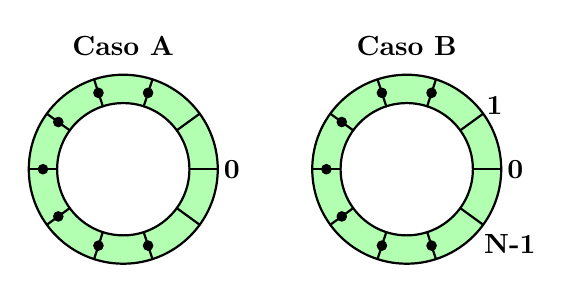
\begin{tikzpicture}[scale=1.2,cap=round,line join=round]
        
        \drawRingC{36,72,108,144,180,216,252,288,324}          {0}{1}{0}{}{}      % no skips
        \node at (0,2.3) {\textbf{Caso A}};
        \drawRingC{0,72,108,144,180,216,252,288}        {3}{1}{0}{1}{N-1}
        \node at (3,2.3) {\textbf{Caso B}};
        % % (Row 2)
        % \drawRing{144,288}    {0}{-6}
        % \drawRing{0,216}      {3}{-6}
        % \drawRing{72,288}     {6}{-6}
        \end{tikzpicture}
        \shorthandon{>}
      \end{center}
Por lo que sin perdida de generalidad se seleccionan estos segmentos la cinta circular la teselación de la siguiente forma:

\textbf{Caso A:} La teselación de la cinta cuando cuando no son unidas las baldosas alrededor de 0:

\begin{center}
    \shorthandoff{>}
  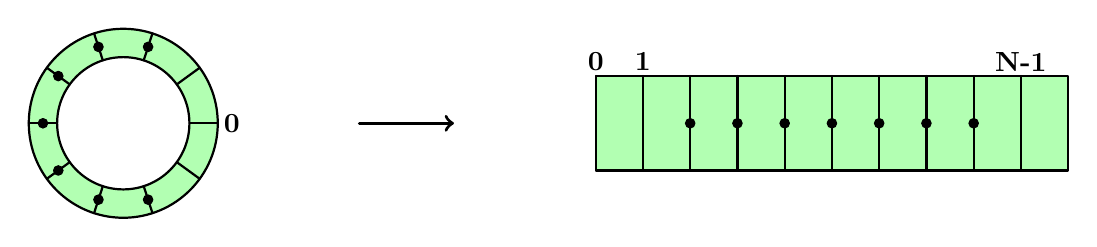
\begin{tikzpicture}[scale=1.2,cap=round,line join=round]
    \drawRingC{36,72,108,144,180,216,252,288,324}          {0}{0}{0}{}{}
    \draw[->, very thick] (2.5,0) -- (3.5,0);
    \drawRectangle{1,2,3,4,5,6,7,8,9}                   {5}{-.5}{0}{1}{N-1}
\end{tikzpicture}
  \shorthandon{>}
\end{center}
Este caso corresponde a contar las formas de telesar la cinta de tamaño \(1 \times n\) con baldosas de tamaño \(1 \times 1\) y \(1 \times 2\). De los ejercicio desarrollados en clase sabemos el numero de formas de teselar es:
\begin{align*}
    t_n = F_{n+1} 
\end{align*}


\textbf{Caso B:} Si la teselación comenzó y finalizo con la misma baldosa $1 \times 2$:
\begin{center}
    \shorthandoff{>}
  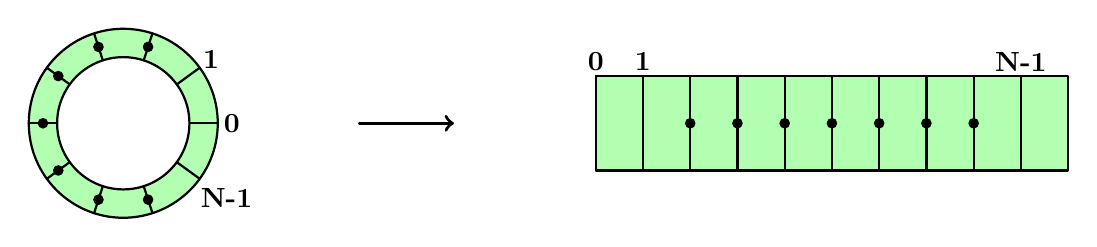
\begin{tikzpicture}[scale=1.2,cap=round,line join=round]
    \drawRingC{0,72,108,144,180,216,252,288}          {0}{0}{0}{1}{N-1}
    \draw[->, very thick] (2.5,0) -- (3.5,0);
    \drawRectangle{1,2,3,4,5,6,7,9}                   {5}{-.5}{0}{1}{N-1}
  \end{tikzpicture}
  \shorthandon{>}
\end{center}

Este caso corresponde a contar las formas de telesar la cinta de tamaño \(1 \times (n-2)\) con baldosas de tamaño \(1 \times 1\) y \(1 \times 2\). De los ejercicio desarrollados en clase sabemos el numero de formas de teselar es:

\begin{align*}
    t_{n-2} = F_{n-1}
\end{align*}

\textbf{Conteo total:} Dado que tenemos dos conteos de casos mutuamente excluyentes, podemos sumar ambos casos para obtener el conteo total de la teselación de la cinta circular de tamaño \(1 \times n\):

\begin{align*}
    c_n = t_n + t_{n-2} = F_{n+1} + F_{n-1}
\end{align*}

\end{solution}